\section{Discrimination des outliers}
Les outliers sont des valeurs qui se situent dans des valeurs extrêmes qui empêche d'obtenir un modèle cohérent.\\
Il est donc important de les identifier et de les exclure pour la suite de l'étude.

\subsection{Méthode de recherche des outliers}

\paragraph{Box Plot}
Pour rechercher les outliers présents dans le jeu de données, une méthode peut consiter à regarder des diagrames en boites à moustaches.
Les valeurs extrèmes apparaissent clairement.

\begin{figure}[H]
	\begin{center}
		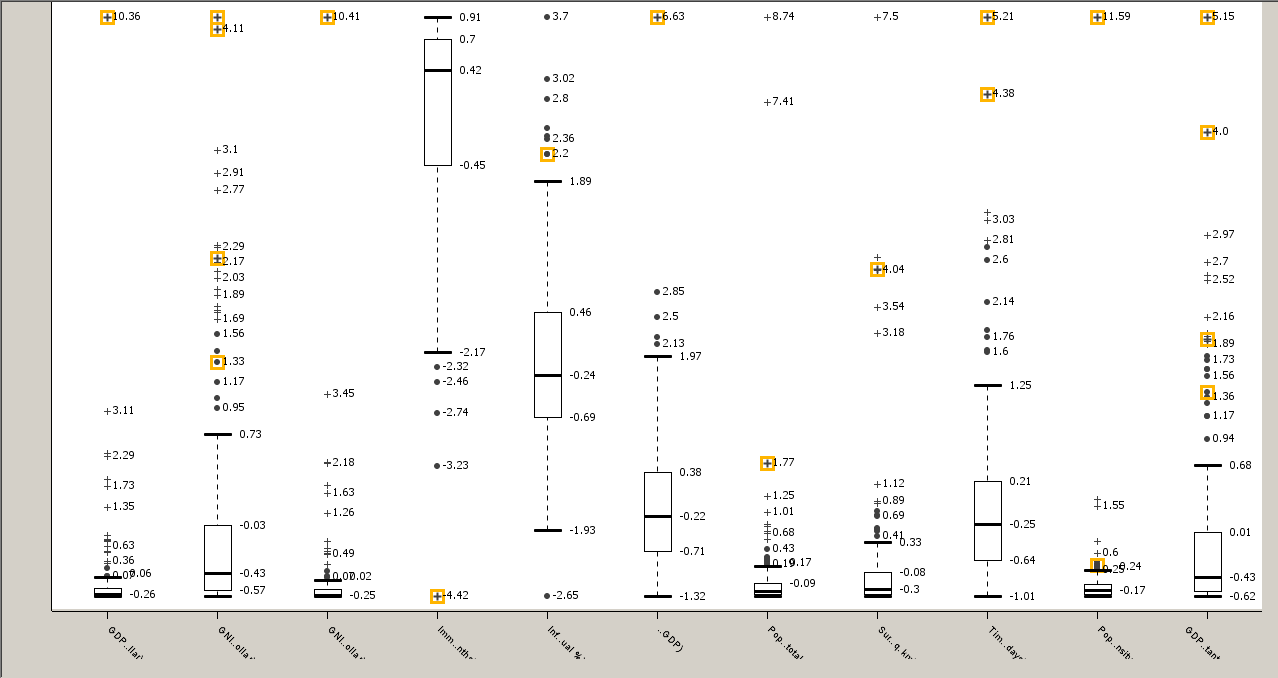
\includegraphics[scale=0.5]{Image/BoxplotOutlierNoMissing2}
		\caption{Diagrammes de boite à moustaches pour le jeu \jeuc}
	\end{center}
\end{figure}

\paragraph{Hierachical trees}
Un autre axe de recherche de ces outliers peut être d'utiliser des clusterisation hierachique en mode SINGLE qui font apraitre les entrée dont les distances sont grandes de façon claires.


\begin{figure}[H]
	\begin{center}
		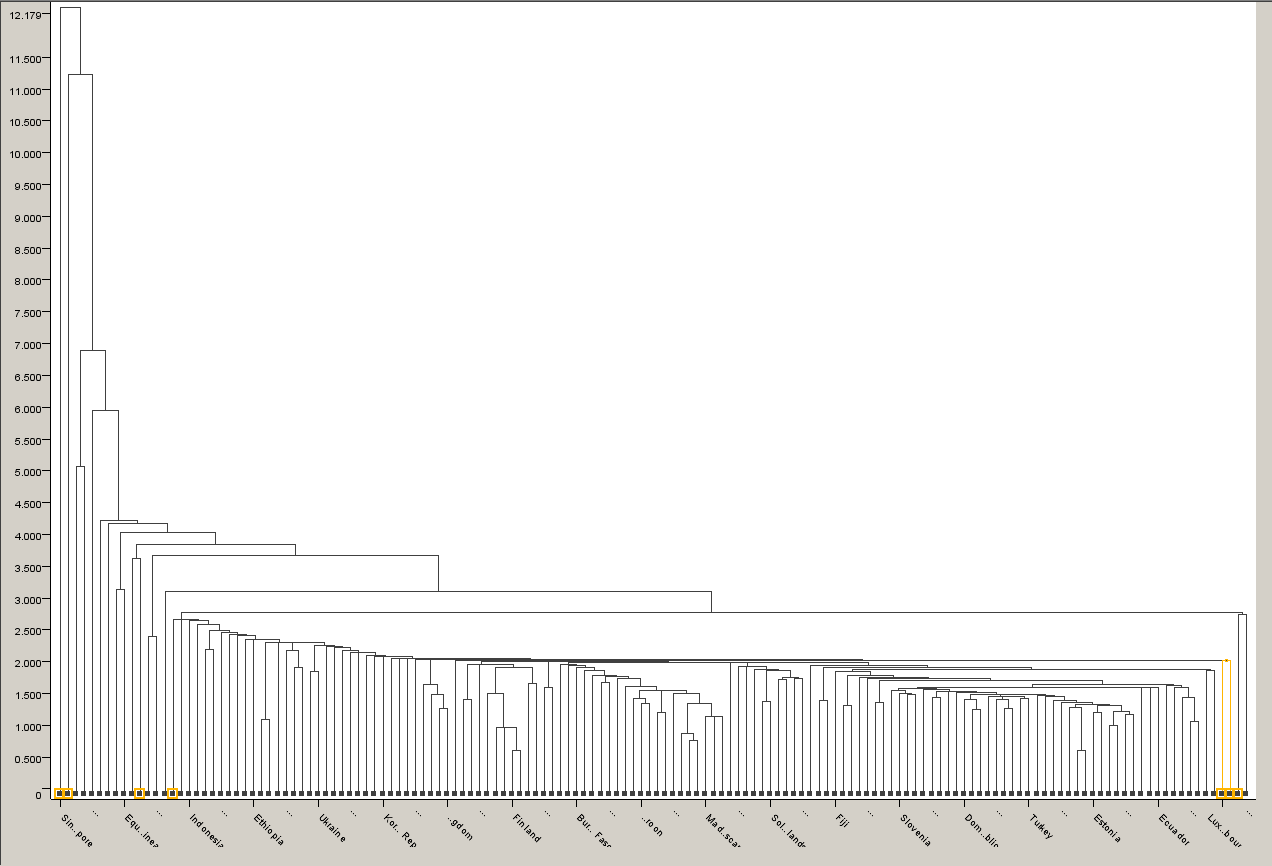
\includegraphics[scale=0.5]{Image/DendogrammeOutliers}
		\caption{Diagrammes de boite à moustaches pour le jeu \jeuc}
	\end{center}
\end{figure}
%hierachical tree en mode single pour trouver les distances "anormales"

\subsection{Outliers écartés}

%liste des outliers écartés